\documentclass{article}
\usepackage{amsmath}
\usepackage{amssymb}
\usepackage{graphicx}
\usepackage{hyperref}
\usepackage[version=4]{mhchem}


\begin{document}
\section*{Problem}
In quadrilateral \(A B C D, A C\) is the angle bisector of \(\angle B A D\). Take \(E\), a point on \(C D\). Connect \(B E\). \(B E\) meets \(A C\) at \(F\). Extend \(D F\) to meet \(B C\) at \(G\). Prove that \(\angle G A C=\angle E A C\).\\
\centering
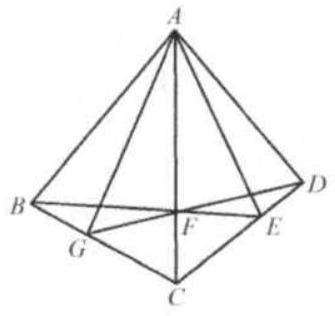
\includegraphics[width=\textwidth]{images/130.jpg}

\section*{Solution}
Draw \(G Q / / C A\) to meet \(B E, B A\) at \(P\) and \(Q\), respectively.\\
Draw \(E S / / C A\) to meet \(D G, D A\) at \(R\) and \(S\), respectively.\\
Connect \(Q S\) to meet \(A C\) at \(M\).\\
Since \(\angle Q A M=\angle S A M, G Q / / C A / / E S\),\\
By the angle bisector theorem, \(\frac{A Q}{A S}=\frac{Q M}{M S}\)\\
We know that \(\triangle P G F \sim \triangle E R F \cdot \frac{P E}{F E}=\frac{G P}{E R}=\frac{G F}{F R}\)\\
We also know that in trapezoid \(G Q S R, \frac{Q M}{M S}=\frac{G F}{F R}\)\\
Thus \(\frac{A Q}{A S}=\frac{Q M}{M S}=\frac{P E}{F E}=\frac{G P}{E R}\)\\
\centering
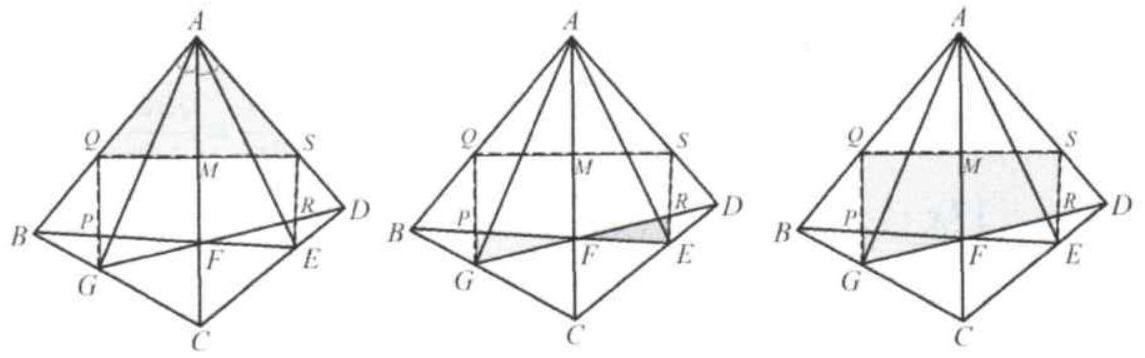
\includegraphics[width=\textwidth]{images/143.jpg}

We know that \(\triangle B G P \sim \triangle B C F \cdot \frac{G P}{C F}=\frac{B G}{B C}\)\\
\centering
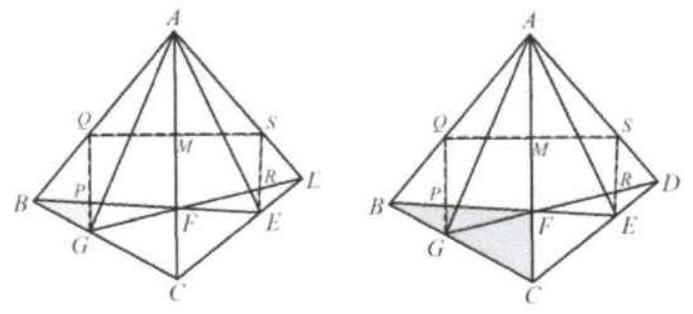
\includegraphics[width=\textwidth]{images/143(1).jpg}


We know that \(\triangle B G Q \sim \triangle B C A \cdot \frac{Q G}{C A}=\frac{B G}{B C}\)\\
\centering
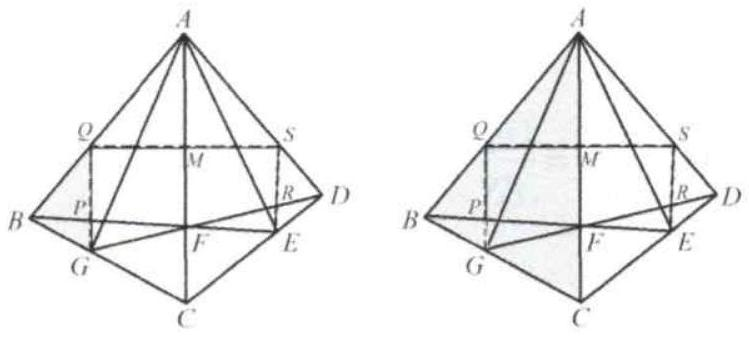
\includegraphics[width=\textwidth]{images/144(2).jpg}

From (5) and (6), we have \(\frac{G P}{C F}=\frac{Q G}{C A} \Rightarrow \frac{G P}{Q G}=\frac{C F}{C A}\)\\
We know that \(\triangle D F C \sim \triangle D R E . \frac{C F}{E R}=\frac{C D}{E D}\)\\
\centering
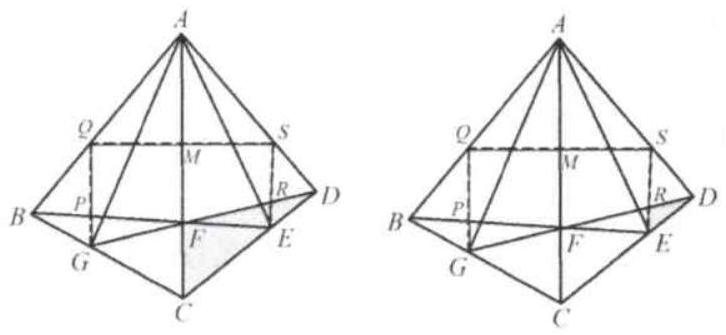
\includegraphics[width=\textwidth]{images/144(1).jpg}

We know that \(\triangle D A C \sim \triangle D S E . \frac{C A}{E S}=\frac{C D}{E D}\)\\
\centering
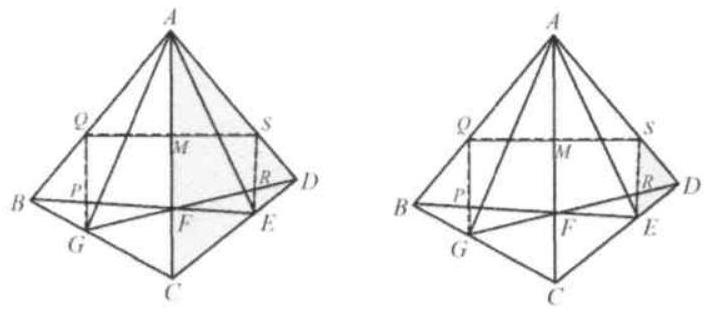
\includegraphics[width=\textwidth]{images/144.jpg}

Combining (8) and (9), \(\frac{C F}{E R}=\frac{C D}{E D}=\frac{C A}{E S} \Rightarrow \frac{C F}{C A}=\frac{E R}{E S}\)

Combining (7) and (10), \(\frac{G P}{G Q}=\frac{C F}{C A}=\frac{E R}{E S} \quad \Rightarrow \quad \frac{G P}{G Q}=\frac{E R}{E S}\)\\
\(\Rightarrow \quad \frac{G P}{E R}=\frac{G Q}{E S}\)\\
Combining (4) and (11), \(\frac{A Q}{A S}=\frac{G Q}{E S}\).\\
\centering
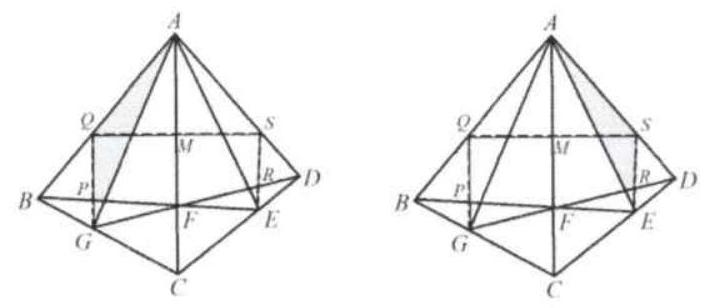
\includegraphics[width=\textwidth]{images/145.jpg}

Since \(A C / / Q G, \angle B A C=\angle B Q G\).\\
Since \(A C / / S E, \angle D A C=\angle D S E\).\\
Since \(\angle B A C=\angle D A C, \angle B Q G=\angle D S E\).\\
\(\angle A Q G=180^{\circ}-\angle B Q G=180^{\circ}-\angle D S E=\angle A S E\),\\
That is, \(\angle A Q G=\angle A S E\).\\
Therefore, \(\triangle A Q G \sim \triangle A S E \quad \Rightarrow \quad \angle Q A G=\angle S A E\).\\
So \(\angle G A C=\angle E A C\).

\section*{Chapter 6 Draw the Auxiliary Lines with Circles}
1. Connect the center of the circle and points on the circumference
\(B\) is the tangent point and \(O\) is the center. Connect \(O B\). We have \(O B \perp A B\).\\
\centering
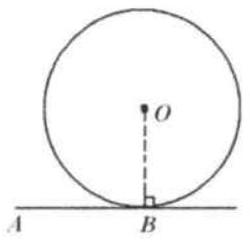
\includegraphics[width=\textwidth]{images/146.jpg}

Theorem 6.1. The radius of a circle is only perpendicular to a tangent line at the point of tangency.

Theorem 6.2. If a line is tangent to a circle, it is perpendicular to a radius at the point of tangency.

Theorem 6.3. A line perpendicular to a radius at a point on the circle is tangent to the circle at that point.

Theorem 6.4. A line perpendicular to a tangent line at the point of tangency with a circle contains the center of the circle.

Theorem 6.5. A line perpendicular to a chord of a circle and containing the center of the circle, bisects the chord and its major and minor arcs.

Theorem 6.6. The perpendicular bisector of a chord of a circle contains the center of the circle.

\end{document}
